\documentclass[aspectratio=169,10pt]{beamer}

\usetheme{Boadilla}
\usecolortheme{seahorse}
\usefonttheme{professionalfonts}

\usepackage[T1]{fontenc}
\usepackage[utf8]{inputenc}
\usepackage{lmodern}
\usepackage{amsmath,amssymb}
\usepackage{graphicx}
\usepackage{booktabs}
\usepackage{siunitx}
\usepackage{xcolor}
\usepackage{hyperref}

\graphicspath{{figures/}}
\setbeamertemplate{navigation symbols}{}
\setbeamertemplate{footline}[frame number]
\setbeamertemplate{caption}[numbered]
\setbeamerfont{frametitle}{series=\bfseries,size=\large}
\setbeamerfont{title}{series=\bfseries,size=\Large}
\setbeamerfont{subtitle}{size=\small}
\setbeamercolor{structure}{fg=blue!45!black}
\setbeamercolor{frametitle}{fg=blue!35!black}

\newcommand{\Bplus}{\ensuremath{B^+}}
\newcommand{\Bminus}{\ensuremath{B^-}}
\newcommand{\ACP}{\ensuremath{A_{\mathrm{CP}}}}
\newcommand{\mevcc}{\ensuremath{\mathrm{MeV}/c^2}}
\newcommand{\gevfour}{\ensuremath{\mathrm{GeV}^2/c^4}}

\title[LHCb Open Data B Decays]{LHCb Open Data Analysis of Three-Body B-Meson Decays}
\subtitle{Invariant-mass reconstruction, signal classification, CP-asymmetry diagnostics and Dalitz-plot studies}
\author{Yanis Idir}
\institute{HEP portfolio project}
\date{\today}

\begin{document}

\begin{frame}
  \titlepage
\end{frame}
% Speaker note: Open with the project goal: a compact, reproducible LHCb Open Data workflow that looks like a real experimental analysis chain.

\begin{frame}{Physics Motivation}
  \begin{columns}[T,onlytextwidth]
    \begin{column}{0.55\textwidth}
      \begin{itemize}
        \item The visible Universe is matter dominated.
        \item CP violation is required but not yet sufficient in the Standard Model.
        \item Heavy-flavour decays probe weak phases and hadronic interference.
      \end{itemize}
    \end{column}
    \begin{column}{0.40\textwidth}
      \begin{block}{Why B mesons?}
        \begin{itemize}
          \item many decay channels
          \item displaced vertices
          \item rich multibody phase space
        \end{itemize}
      \end{block}
    \end{column}
  \end{columns}
\end{frame}
% Speaker note: Emphasize that this is a motivation slide, not a full theory review: B decays are a practical lab for CP and flavour studies.

\begin{frame}{LHCb Experiment and Dataset}
  \begin{columns}[T,onlytextwidth]
    \begin{column}{0.52\textwidth}
      \begin{itemize}
        \item LHCb: forward spectrometer at the LHC.
        \item Optimized for beauty and charm hadrons.
        \item Excellent tracking, vertexing and particle identification.
      \end{itemize}
    \end{column}
    \begin{column}{0.43\textwidth}
      \begin{block}{Input sample}
        \begin{itemize}
          \item CERN Open Data
          \item ROOT files
          \item \texttt{DecayTree} TTree
          \item track momenta, charge, PID, vertex variables
        \end{itemize}
      \end{block}
    \end{column}
  \end{columns}
\end{frame}
% Speaker note: Point out that the project starts from realistic HEP ntuples rather than toy CSV files.

\begin{frame}{Analysis Workflow}
  \centering
  \vspace{0.2cm}
  {\large
  ROOT \(\rightarrow\) \texttt{uproot} \(\rightarrow\) \texttt{pandas}
  \(\rightarrow\) reconstruction \(\rightarrow\) cuts
  \(\rightarrow\) ML \(\rightarrow\) physics observables}

  \vspace{0.8cm}
  \begin{columns}[T,onlytextwidth]
    \begin{column}{0.30\textwidth}
      \begin{block}{Data}
        Branch loading\\
        candidate tables\\
        reproducible paths
      \end{block}
    \end{column}
    \begin{column}{0.30\textwidth}
      \begin{block}{Physics}
        invariant mass\\
        event selection\\
        charge split
      \end{block}
    \end{column}
    \begin{column}{0.30\textwidth}
      \begin{block}{Outputs}
        figures\\
        ML diagnostics\\
        CP and Dalitz studies
      \end{block}
    \end{column}
  \end{columns}
\end{frame}
% Speaker note: This slide is the roadmap; mention that reusable functions live under src/ and notebooks only orchestrate analysis steps.

\begin{frame}{Invariant-Mass Reconstruction}
  \begin{columns}[T,onlytextwidth]
    \begin{column}{0.50\textwidth}
      \begin{block}{Three-kaon hypothesis}
        \[
          E_i = \sqrt{p_{x,i}^2+p_{y,i}^2+p_{z,i}^2+m_K^2}
        \]
        \[
          m_B^2 =
          \left(\sum_i E_i\right)^2
          -
          \left|\sum_i \vec{p}_i\right|^2
        \]
      \end{block}
    \end{column}
    \begin{column}{0.45\textwidth}
      \begin{itemize}
        \item assign \(m_K=493.677~\mevcc\)
        \item build daughter four-vectors
        \item sum to reconstruct B candidate
        \item vectorized in \texttt{numpy}/\texttt{pandas}
      \end{itemize}
    \end{column}
  \end{columns}
\end{frame}
% Speaker note: Keep the formula intuitive: the entire mass reconstruction is a four-vector sum under a kaon mass hypothesis.

\begin{frame}{Mass Spectrum and Signal Fit}
  \begin{columns}[T,onlytextwidth]
    \begin{column}{0.49\textwidth}
      \centering
      {\scriptsize B-candidate mass after baseline selection}\\[-0.05cm]
      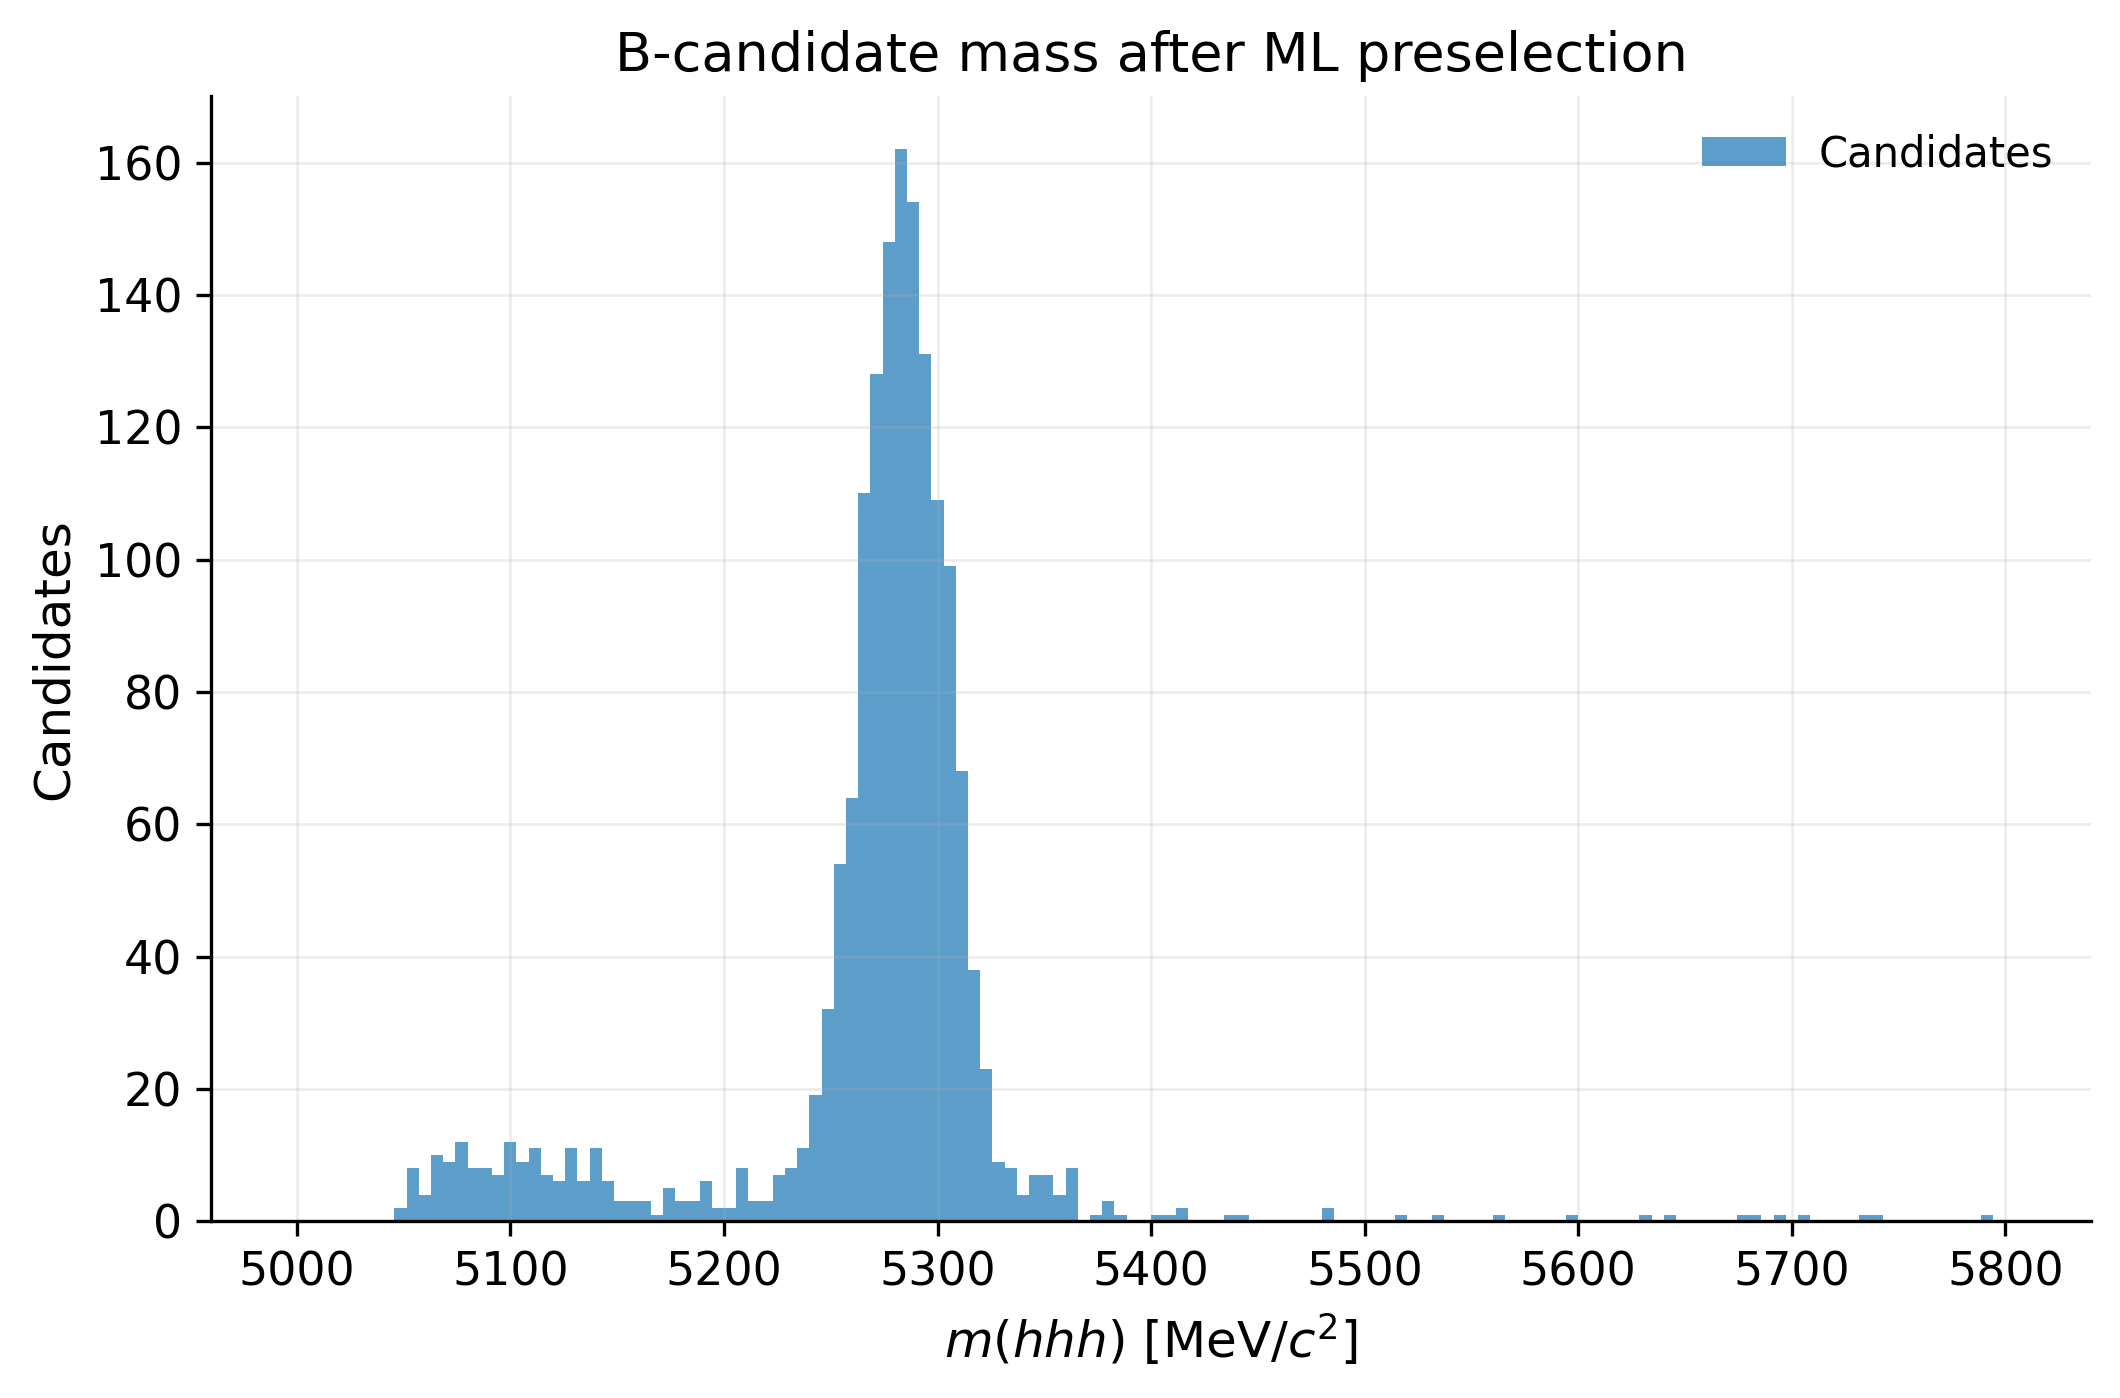
\includegraphics[width=\textwidth,trim=0 0 0 42,clip]{B_mass_after_cuts.png}
      \vspace{0.05cm}
      {\scriptsize Selected candidates}
    \end{column}
    \begin{column}{0.49\textwidth}
      \centering
      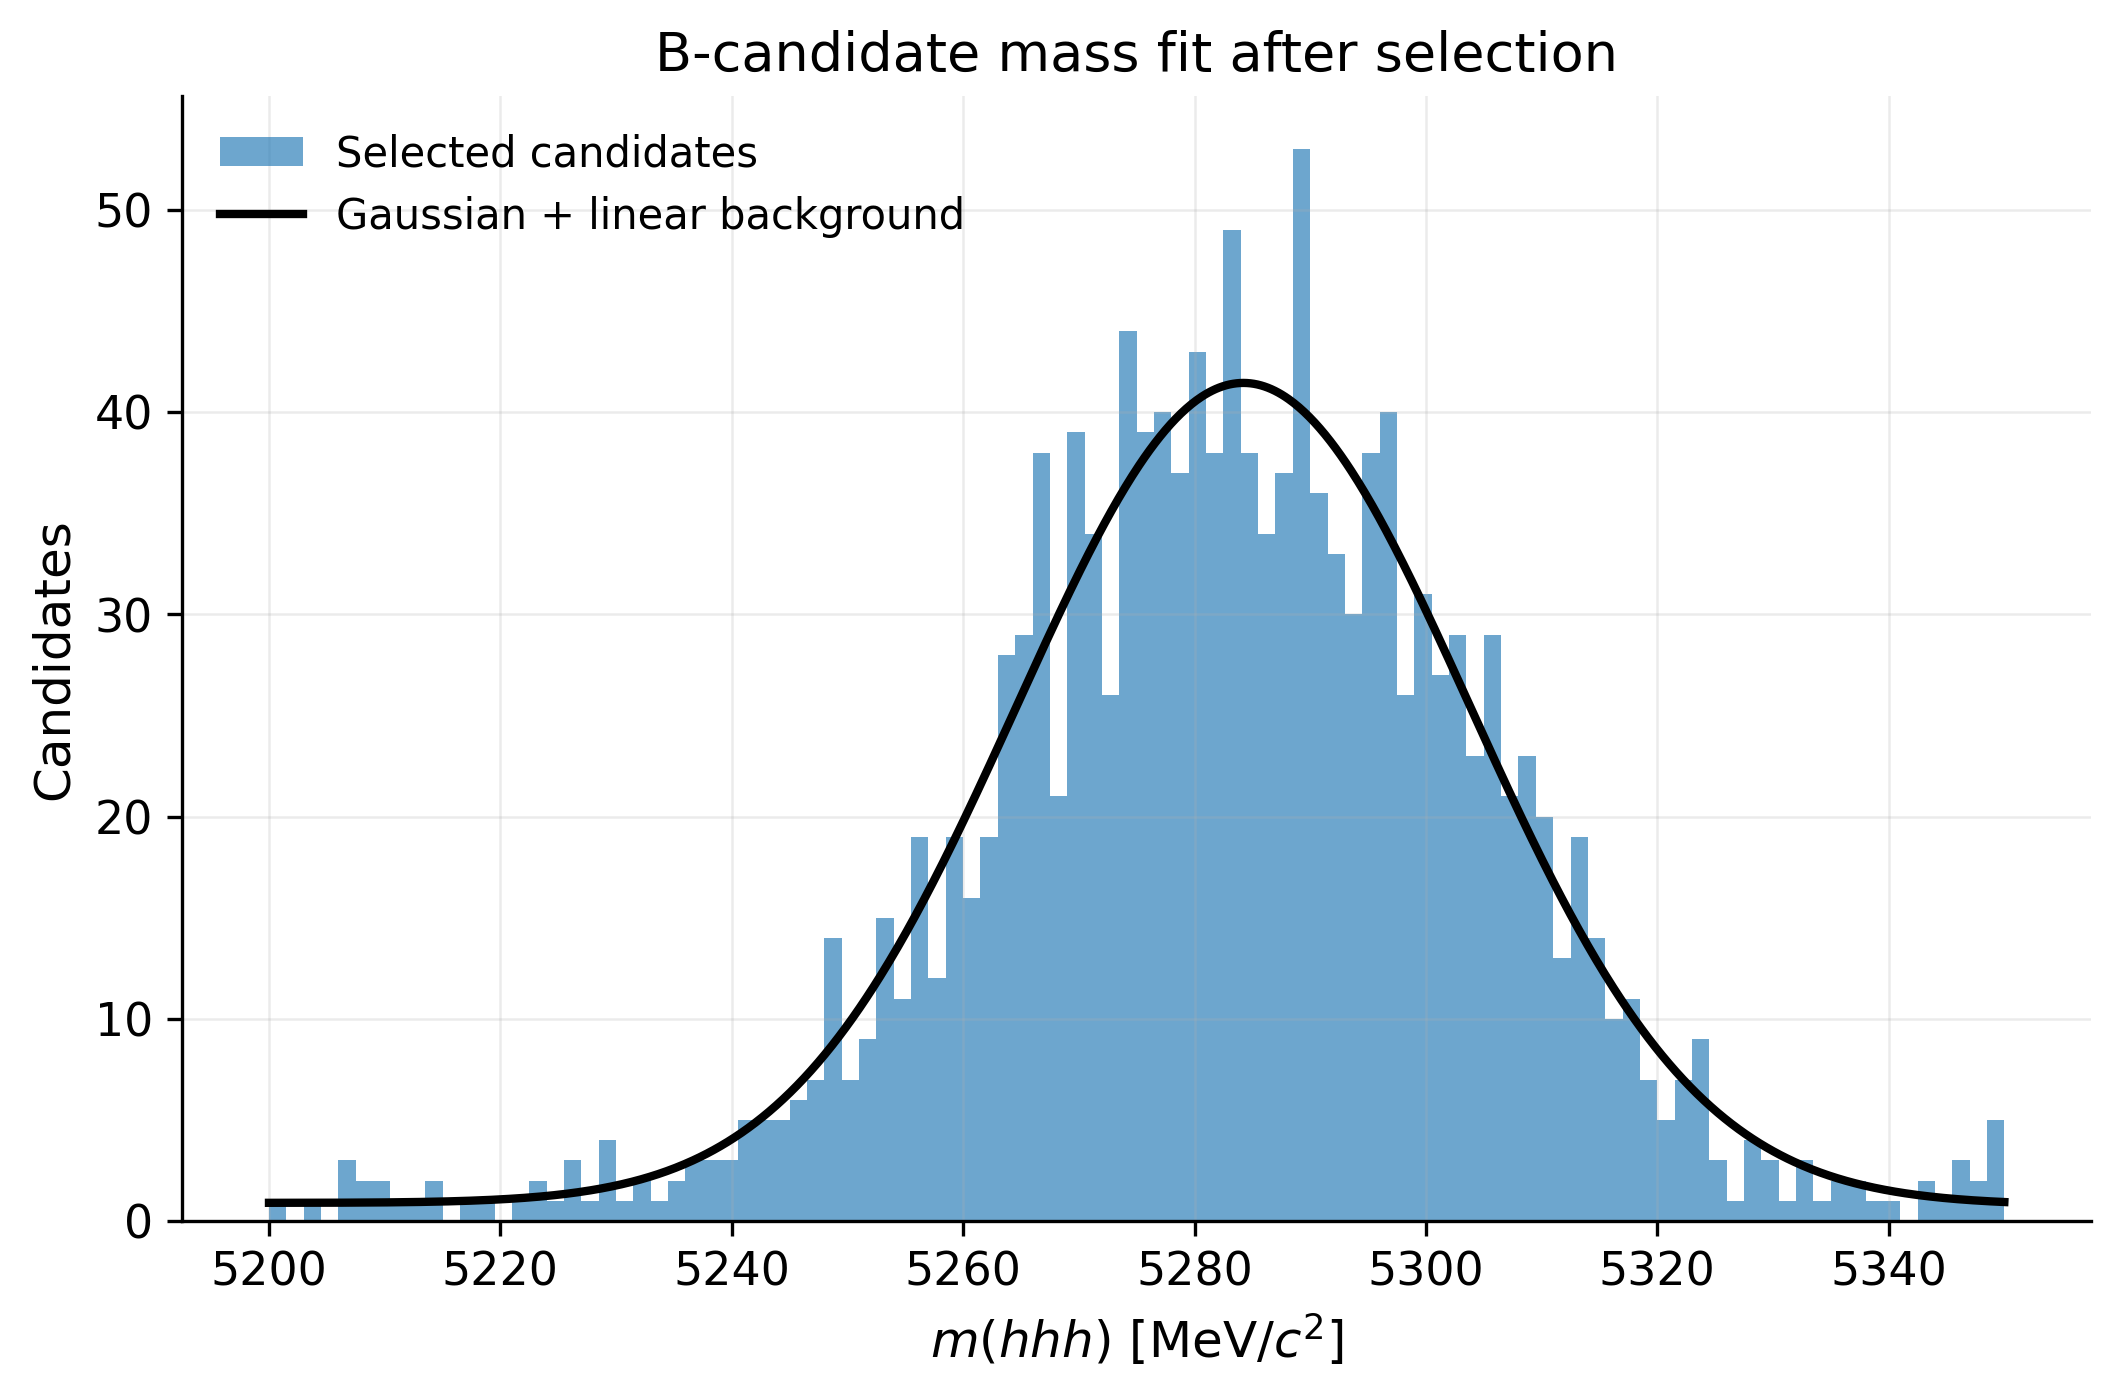
\includegraphics[width=\textwidth]{B_mass_fit.png}
      \vspace{0.05cm}
      {\scriptsize Gaussian + linear background}
    \end{column}
  \end{columns}
  \vspace{0.15cm}
  \[
    f(m)=A e^{-(m-\mu)^2/(2\sigma^2)} + a m + b
  \]
\end{frame}
% Speaker note: Highlight that the peak validates the reconstruction and gives a simple signal-extraction benchmark.

\begin{frame}{Event Selection}
  \begin{columns}[T,onlytextwidth]
    \begin{column}{0.45\textwidth}
      \begin{block}{Baseline cuts}
        \[
          \chi^2_{\mathrm{vtx}}(B) < 5
        \]
        \[
          d_{\mathrm{flight}}(B) > 20
        \]
        \[
          P_K(H_1),P_K(H_2),P_K(H_3) > 0.5
        \]
      \end{block}
    \end{column}
    \begin{column}{0.50\textwidth}
      \begin{itemize}
        \item vertex quality: common displaced decay point
        \item flight distance: B lifetime signature
        \item kaon PID: consistency with \(B\to KKK\)
        \item same cuts reused across notebooks
      \end{itemize}
    \end{column}
  \end{columns}
\end{frame}
% Speaker note: Stress that these cuts are intentionally simple, interpretable and shared across the analysis.

\begin{frame}{Signal/Background Classification}
  \begin{columns}[T,onlytextwidth]
    \begin{column}{0.49\textwidth}
      \centering
      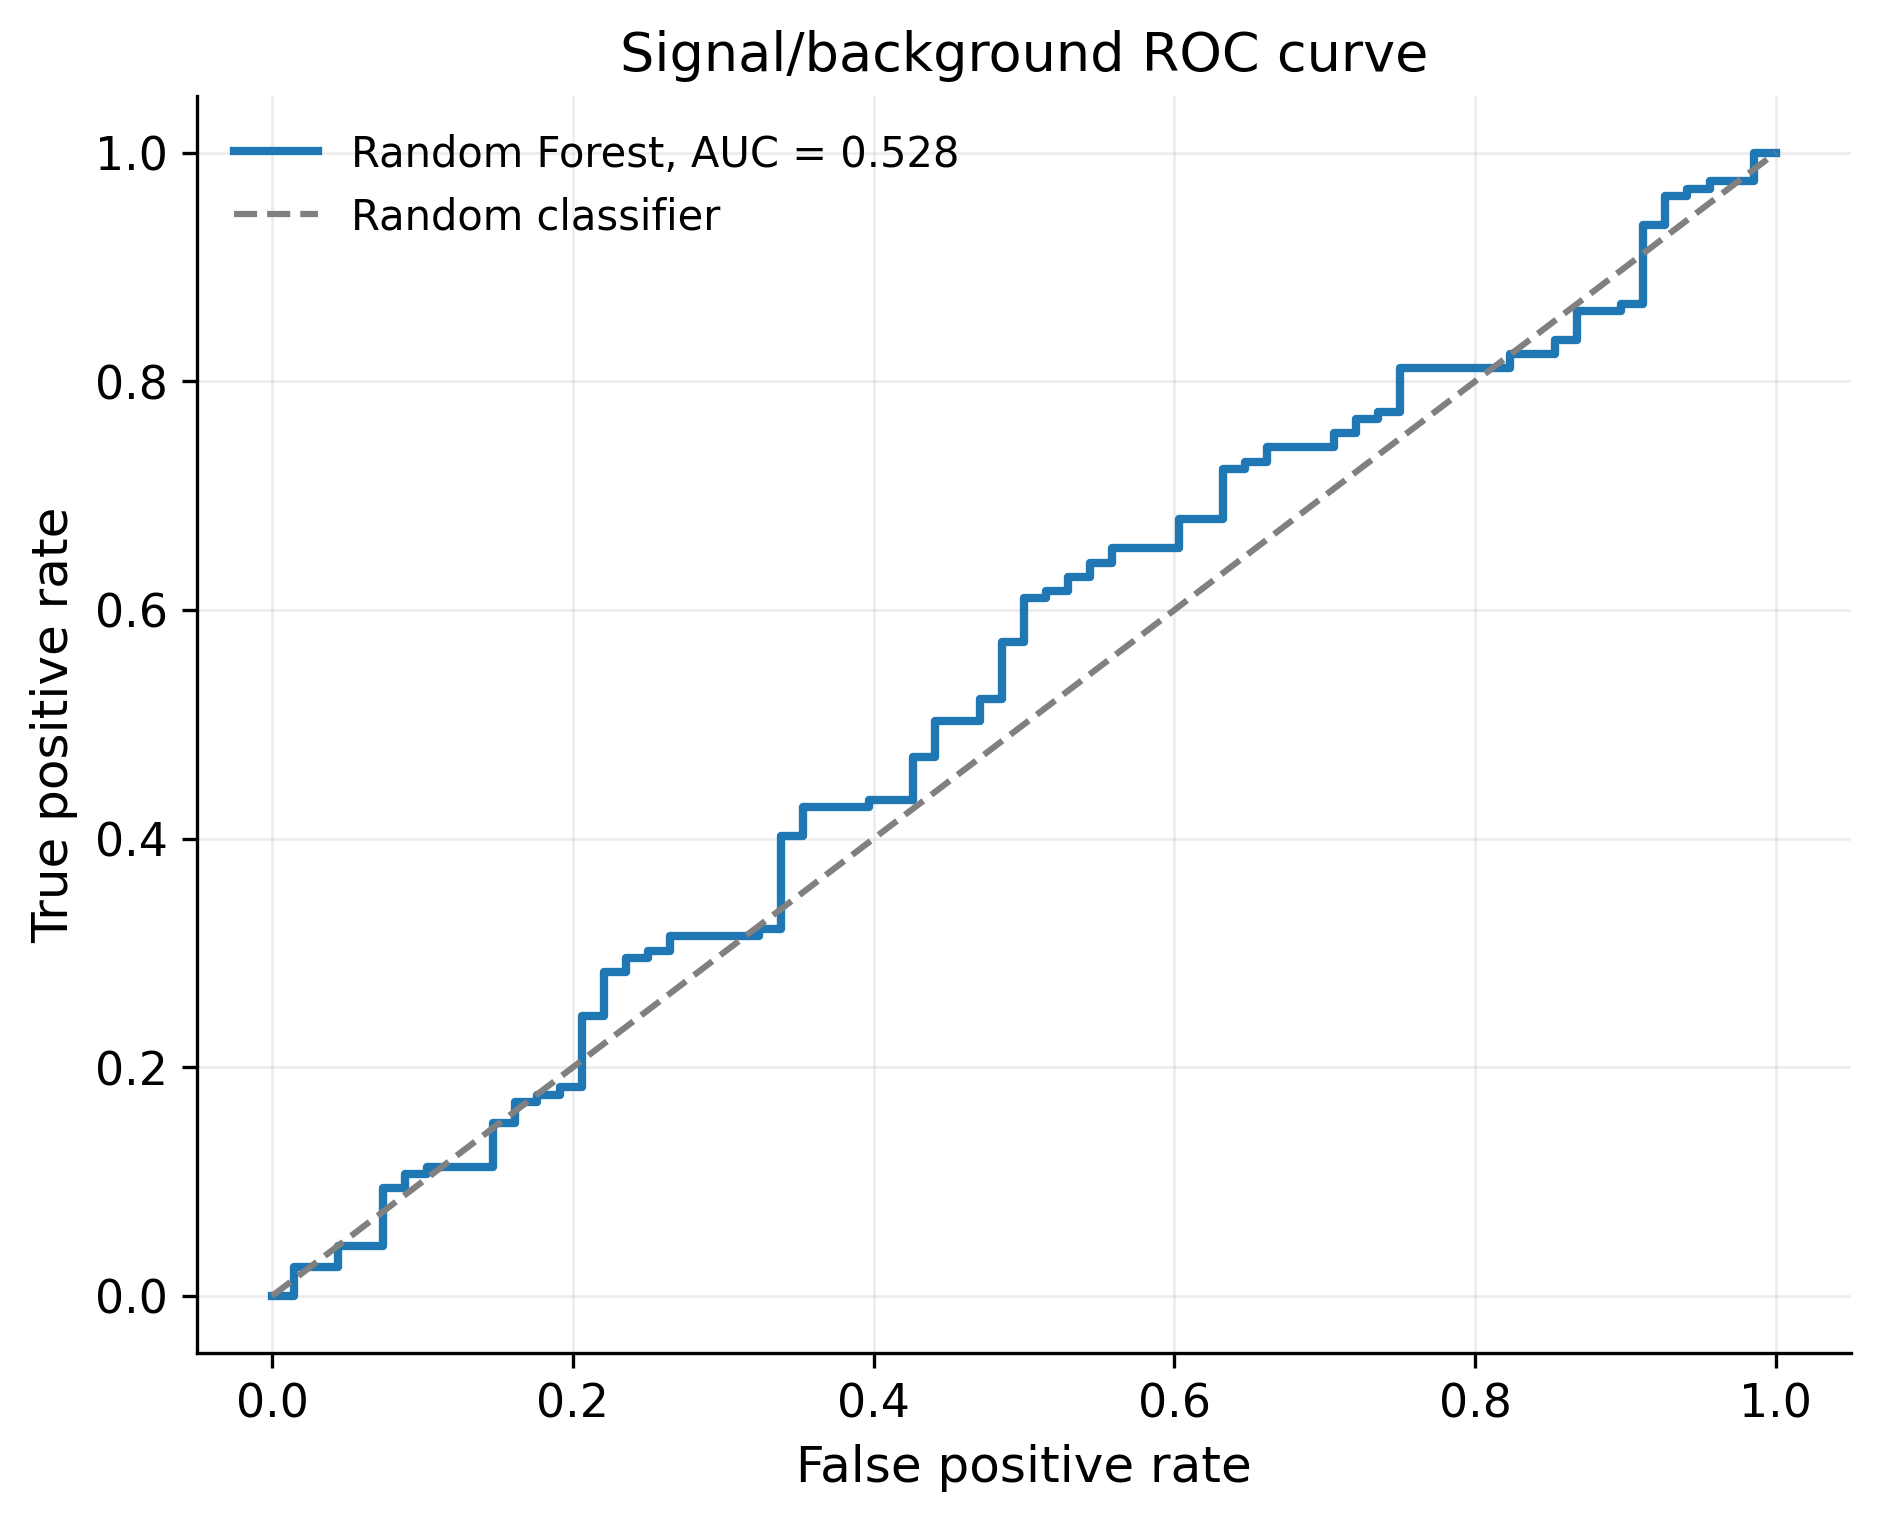
\includegraphics[width=0.94\textwidth]{roc_signal_background.png}
    \end{column}
    \begin{column}{0.49\textwidth}
      \centering
      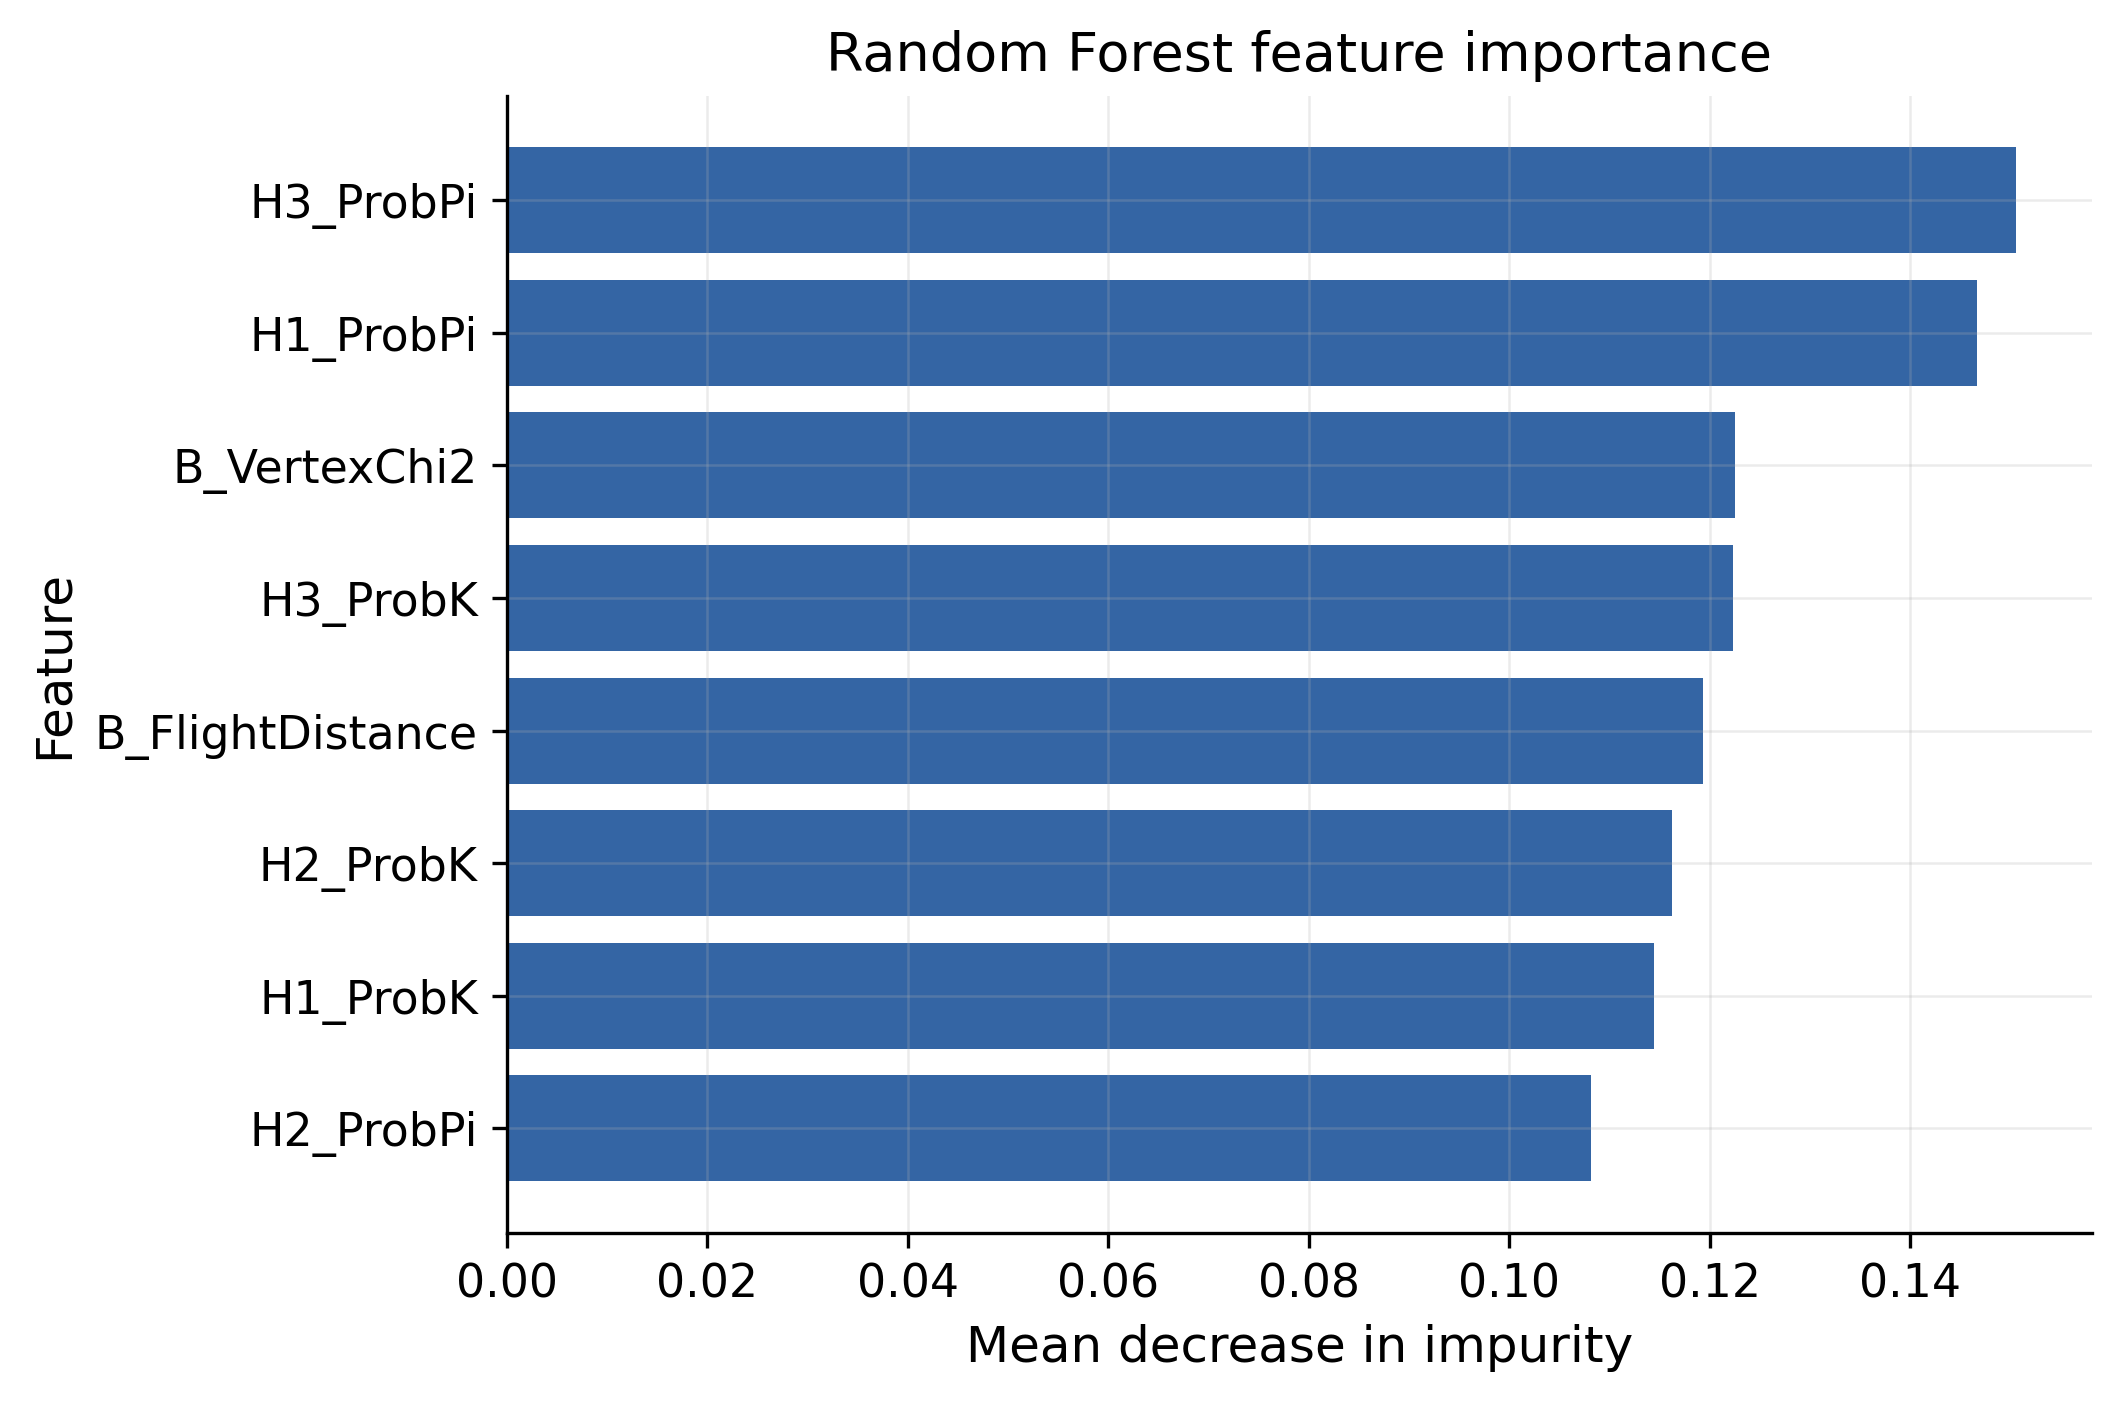
\includegraphics[width=0.94\textwidth]{feature_importance_signal_background.png}
    \end{column}
  \end{columns}
  \vspace{0.05cm}
  \begin{itemize}
    \item Sideband-labelled Random Forest classifier.
    \item AUC is a diagnostic of separation power, not the main physics result.
  \end{itemize}
  {\footnotesize The low AUC indicates limited residual separation after the baseline cuts, not a failure of the physics reconstruction.}
\end{frame}
% Speaker note: Make clear that the classifier excludes mass to avoid learning the label definition directly.

\begin{frame}{CP-Asymmetry Diagnostic}
  \begin{columns}[T,onlytextwidth]
    \begin{column}{0.50\textwidth}
      \[
        \ACP^{\mathrm{raw}} =
        \frac{N(\Bminus)-N(\Bplus)}
             {N(\Bminus)+N(\Bplus)}
      \]
      \begin{itemize}
        \item signal window: \(5270<m_B<5290~\mevcc\)
        \item \(N(\Bplus)=282,\quad N(\Bminus)=246\)
        \item \(\ACP^{\mathrm{raw}}=-0.06818\)
      \end{itemize}
      {\small Not corrected for detector or production effects.}
    \end{column}
    \begin{column}{0.48\textwidth}
      \centering
      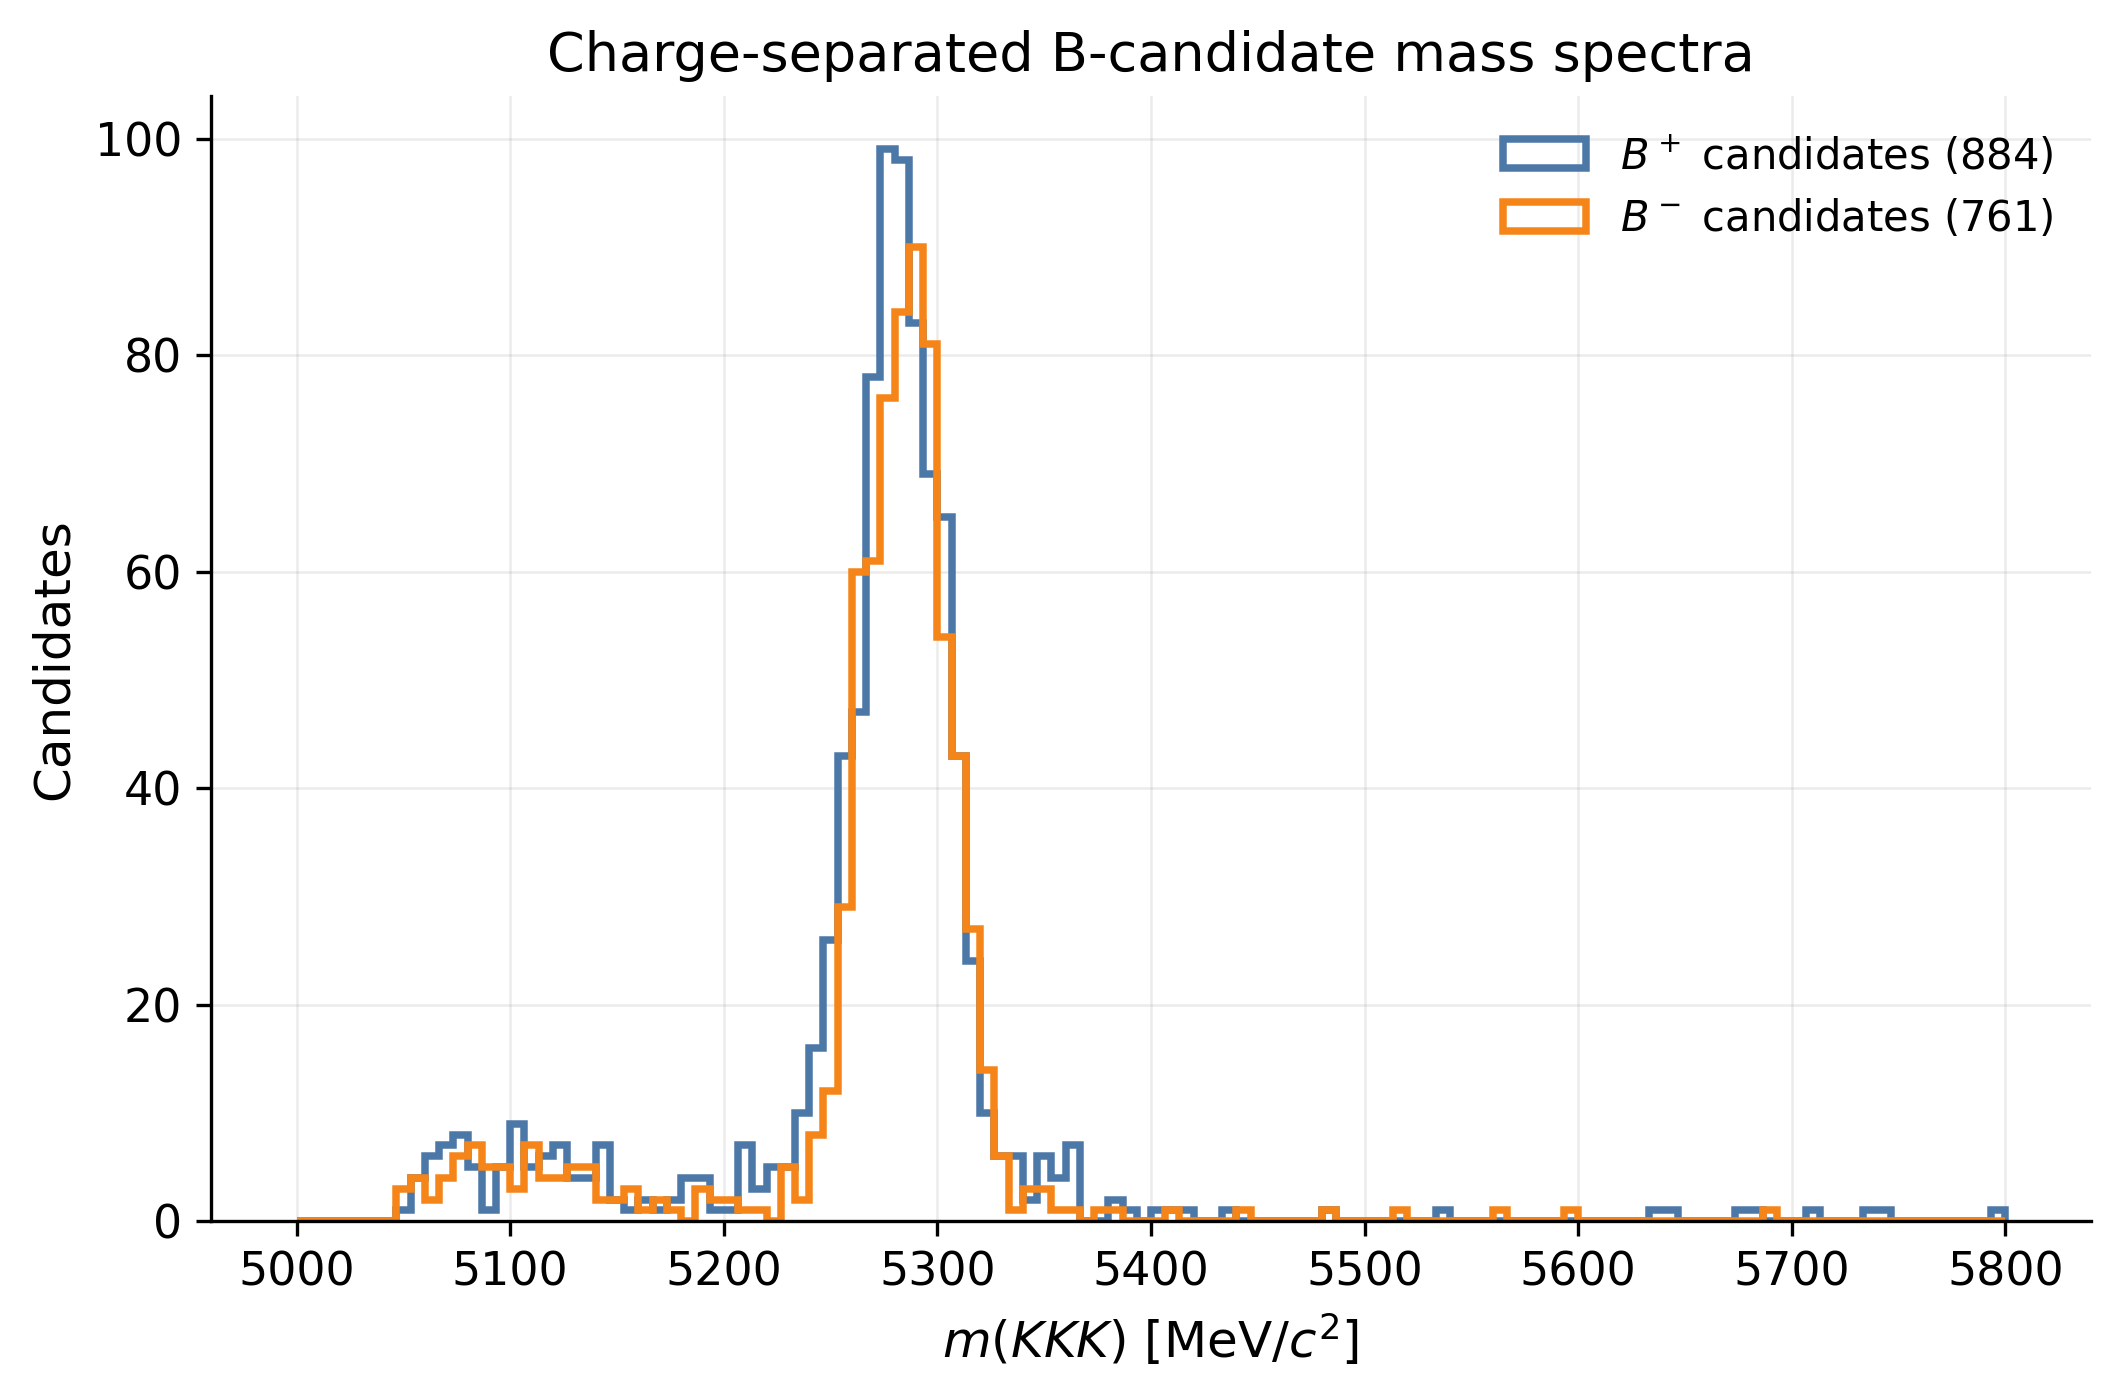
\includegraphics[width=\textwidth]{cp_mass_overlay.png}
    \end{column}
  \end{columns}
\end{frame}
% Speaker note: State explicitly that this is a raw diagnostic and not a publishable CP measurement.

\begin{frame}{Dalitz-Plot Analysis}
  \begin{columns}[T,onlytextwidth]
    \begin{column}{0.43\textwidth}
      \begin{itemize}
        \item Pairwise invariant masses:
      \end{itemize}
      \[
        m_{ij}^2=(E_i+E_j)^2-
        |\vec{p}_i+\vec{p}_j|^2
      \]
      \begin{itemize}
        \item \(m^2(K_1K_2)\)
        \item \(m^2(K_2K_3)\)
        \item \(m^2(K_1K_3)\)
      \end{itemize}
      {\small Useful for resonance and local CP studies.}
    \end{column}
    \begin{column}{0.55\textwidth}
      \centering
      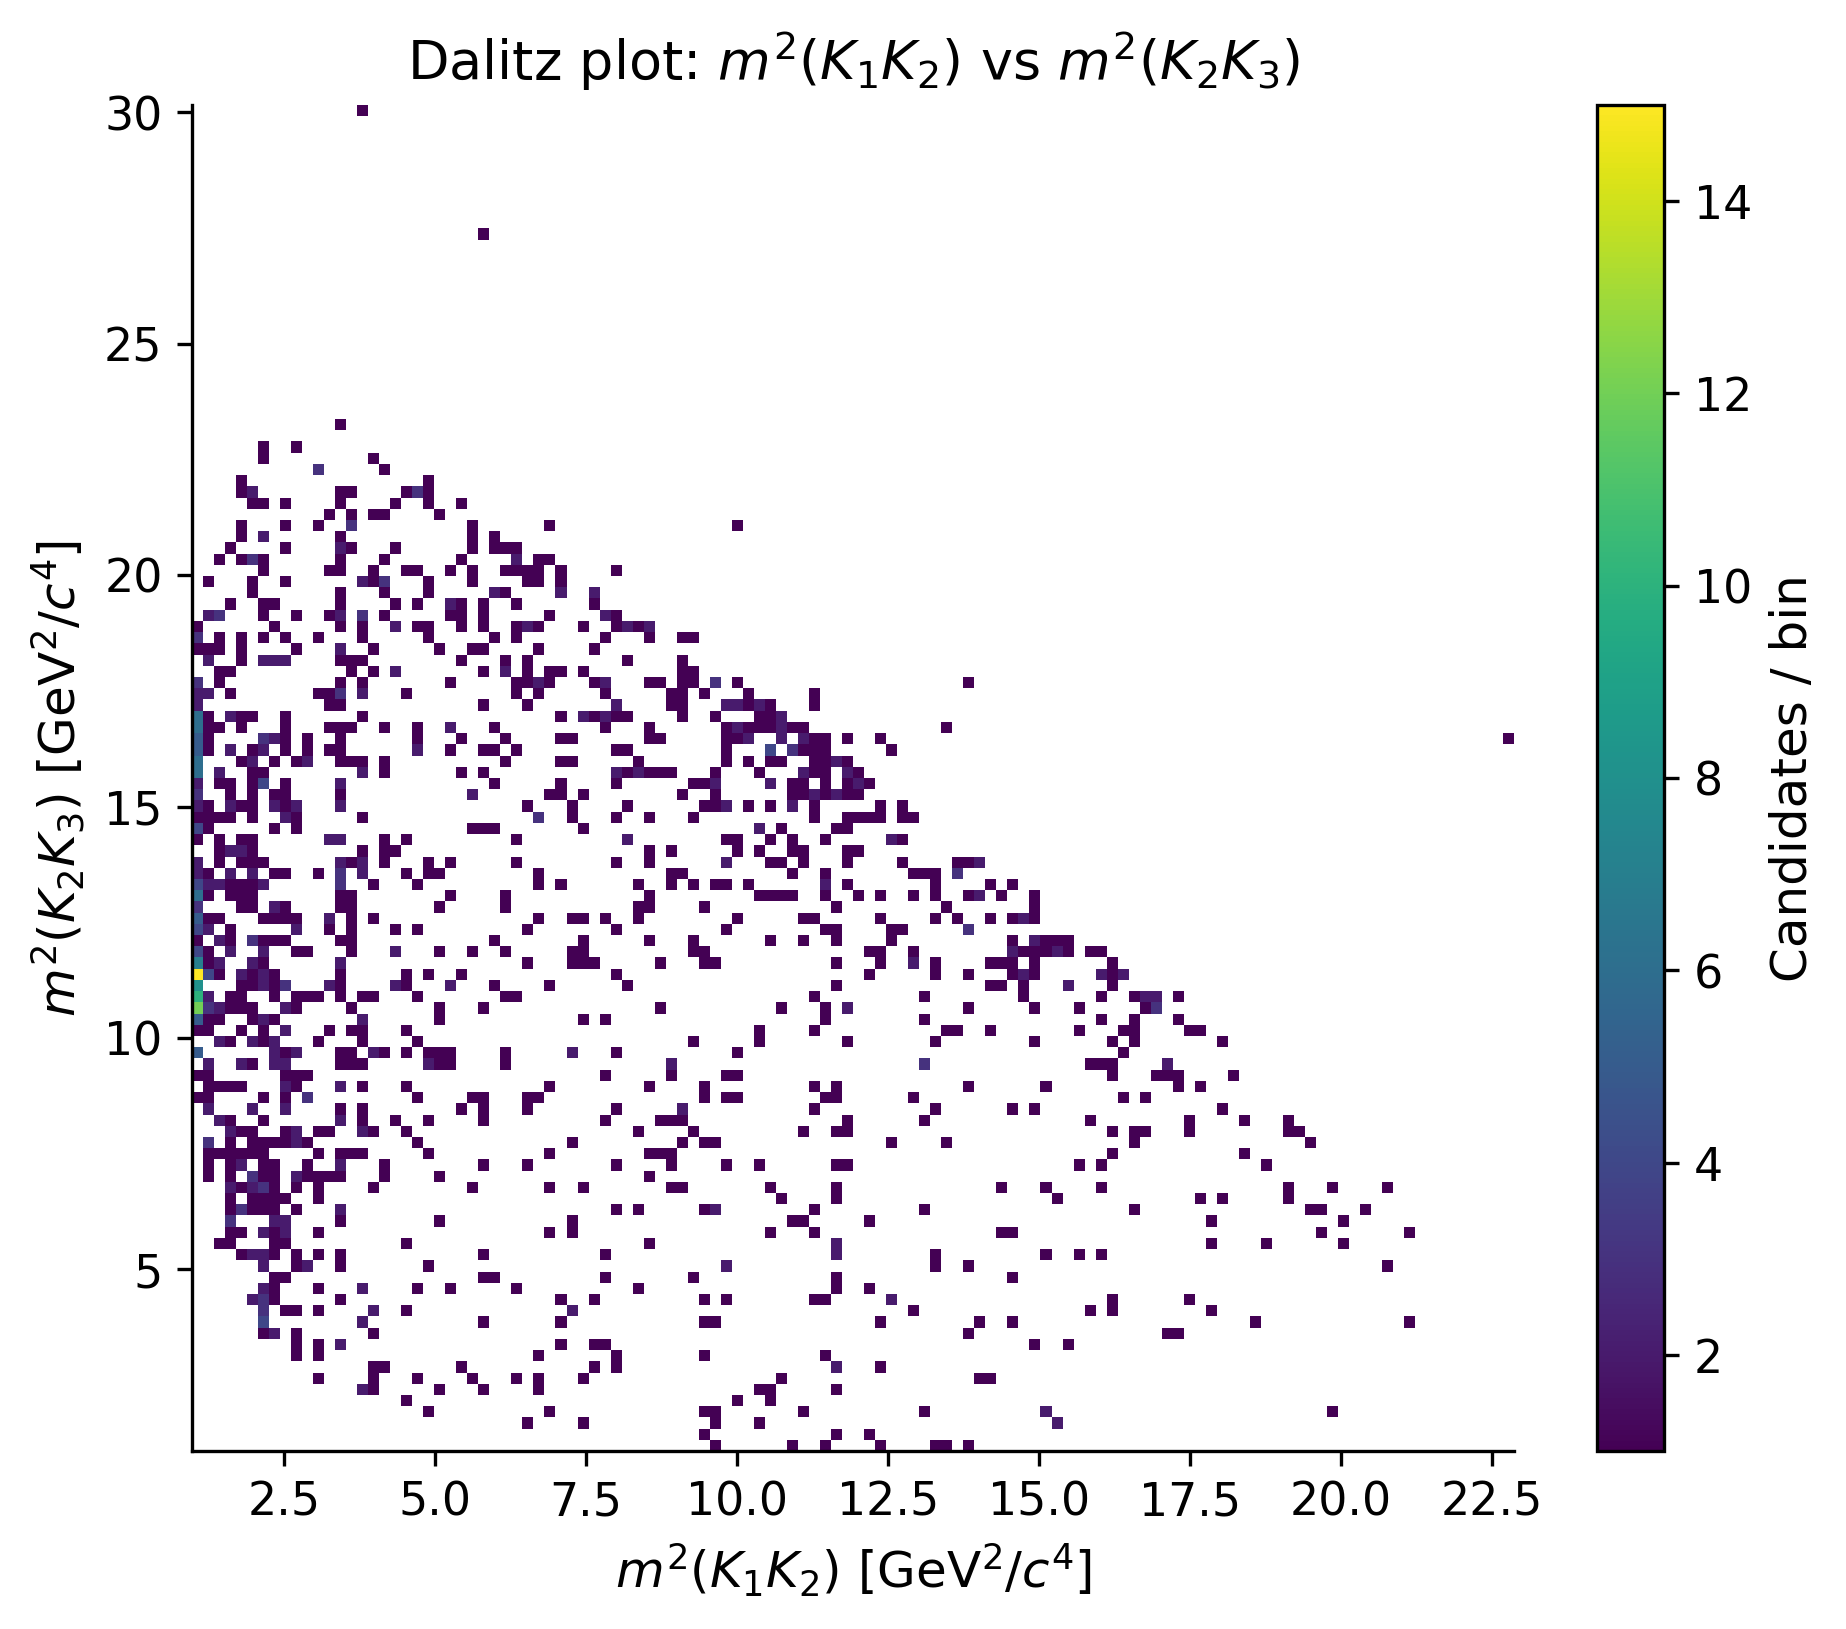
\includegraphics[width=0.49\textwidth]{dalitz_mK1K2_vs_mK2K3.png}
      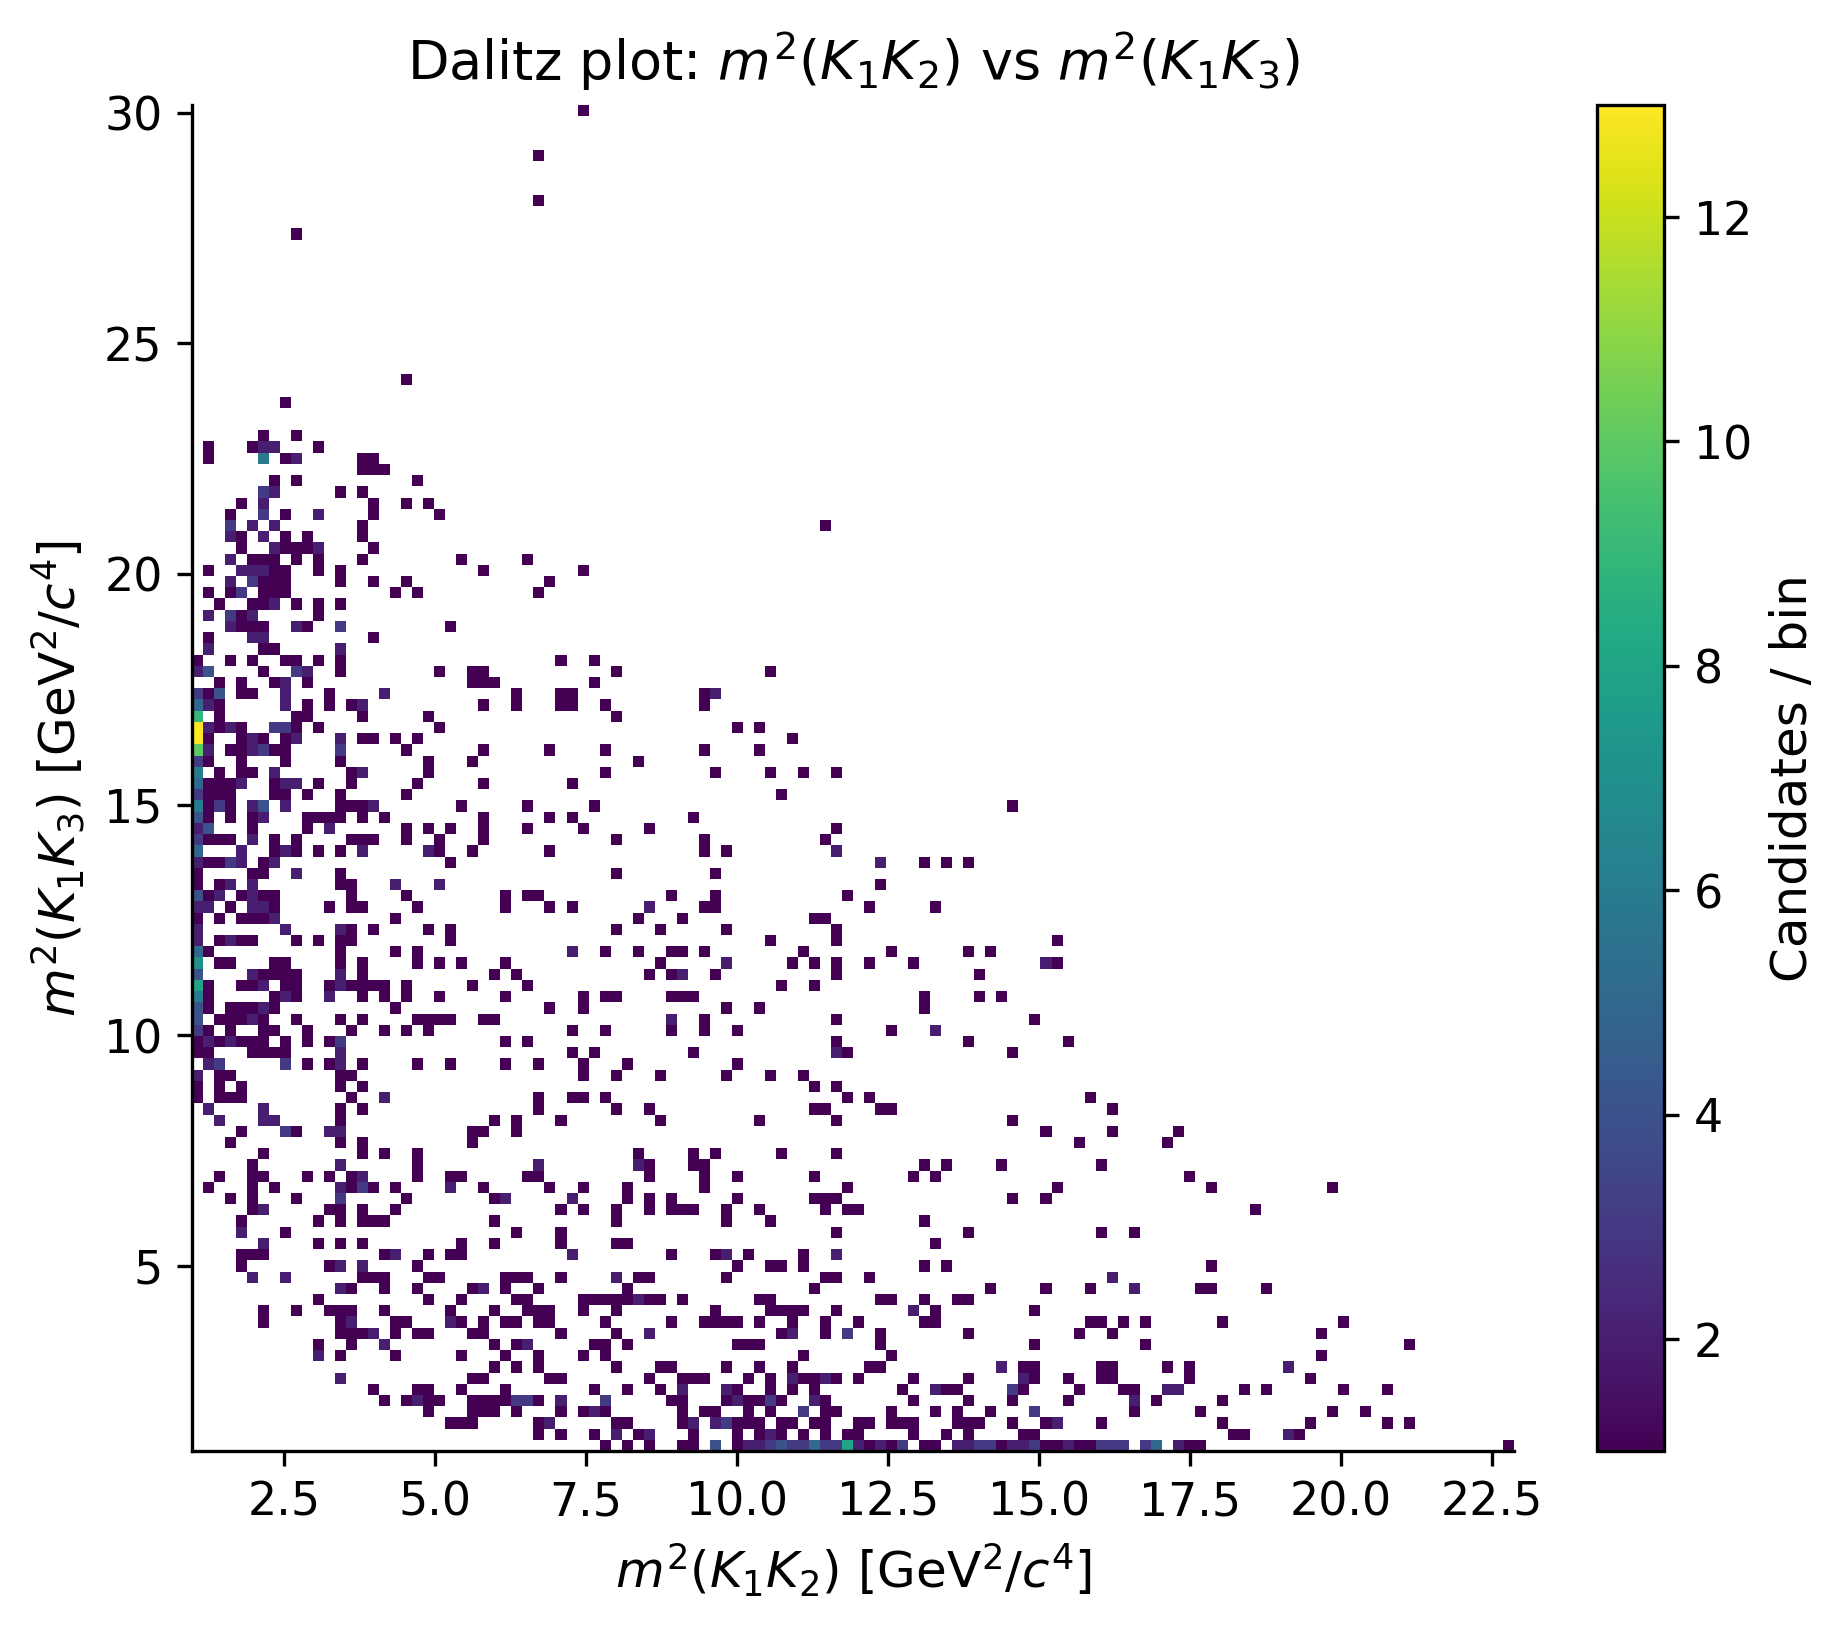
\includegraphics[width=0.49\textwidth]{dalitz_mK1K2_vs_mK1K3.png}
    \end{column}
  \end{columns}
\end{frame}
% Speaker note: Explain that Dalitz plots reveal phase-space structure beyond the one-dimensional B mass.

\begin{frame}{Limitations and Future Work}
  \begin{columns}[T,onlytextwidth]
    \begin{column}{0.48\textwidth}
      \begin{block}{Current limitations}
        \begin{itemize}
          \item raw asymmetry only
          \item single-polarity demonstration
          \item simple mass model
          \item sideband proxy labels
        \end{itemize}
      \end{block}
    \end{column}
    \begin{column}{0.48\textwidth}
      \begin{block}{Next steps}
        \begin{itemize}
          \item combine MagnetUp/MagnetDown
          \item detector corrections and simulation
          \item XGBoost or boosted decision trees
          \item local CP asymmetries in Dalitz bins
        \end{itemize}
      \end{block}
    \end{column}
  \end{columns}
\end{frame}
% Speaker note: This is where to show maturity: the project is strong because it names what would be needed for a real measurement.

\begin{frame}{Conclusion}
  \begin{itemize}
    \item Reproducible HEP workflow from ROOT ntuples to physics plots.
    \item Invariant-mass reconstruction under a kaon mass hypothesis.
    \item Shared selections and modular Python functions.
    \item Sideband ML diagnostics, raw CP-asymmetry study and Dalitz plots.
  \end{itemize}

  \vspace{0.5cm}
  \begin{center}
    \Large \textbf{A compact portfolio analysis mirroring a real LHCb workflow}
  \end{center}
\end{frame}
% Speaker note: End by connecting the technical work to readiness for an experimental HEP PhD environment.

\end{document}
